% Nejprve uvedeme tridu dokumentu s volbami
\documentclass[czech,master,dept460,male,cpp,cpdeclaration,oneside]{diploma}
% Dalsi doplnujici baliky maker
\usepackage[autostyle=true,czech=quotes]{csquotes} % korektni sazba uvozovek, podpora pro balik biblatex
\usepackage[backend=biber, style=iso-numeric, alldates=iso, autocite = superscript]{biblatex} % bibliografie
\usepackage{dcolumn} % sloupce tabulky s ciselnymi hodnotami
\usepackage{subfig} % makra pro "podobrazky" a "podtabulky"


% Custom packages
\usepackage{hyperref}
\usepackage[utf8]{inputenc}
\usepackage{amsmath}
\usepackage{amssymb}
\usepackage{color}
\usepackage{listings}
\usepackage{xcolor}
\usepackage[bottom]{footmisc}
\usepackage{upquote}
\usepackage{underscore}
\usepackage{afterpage}
\usepackage{array}
\usepackage{comment}
\usepackage{float}
\usepackage{setspace}

% Definitions

\definecolor{dkgreen}{rgb}{0,0.6,0}
\definecolor{ltgray}{rgb}{0.5,0.5,0.5}

\definecolor{eclipseStrings}{RGB}{42,0.0,255}
\definecolor{eclipseKeywords}{RGB}{127,0,85}
\colorlet{numb}{magenta!60!black}

\definecolor{lightgray}{rgb}{.9,.9,.9}
\definecolor{darkgray}{rgb}{.4,.4,.4}
\definecolor{purple}{rgb}{0.65, 0.12, 0.82}

\definecolor{mediumgray}{rgb}{0.3, 0.4, 0.4}
\definecolor{mediumblue}{rgb}{0.0, 0.0, 0.8}
\definecolor{forestgreen}{rgb}{0.13, 0.55, 0.13}
\definecolor{darkviolet}{rgb}{0.58, 0.0, 0.83}
\definecolor{royalblue}{rgb}{0.25, 0.41, 0.88}
\definecolor{crimson}{rgb}{0.86, 0.8, 0.24}

\tolerance=1
\emergencystretch=\maxdimen
\hyphenpenalty=10000
\hbadness=10000
\setstretch{1.08}

\lstset{
	basicstyle=\fontsize{10}{12}\selectfont\ttfamily
}

\lstdefinelanguage{json}{
	basicstyle=\normalfont\ttfamily,
	commentstyle=\color{eclipseStrings}, % style of comment
	stringstyle=\color{eclipseKeywords}, % style of strings
	numbersep=8pt,
	showstringspaces=false,
	breaklines=true,
	frame=lines,
	string=[s]{"}{"},
	comment=[l]{:\ "},
	morecomment=[l]{:"},
	literate=
	*{0}{{{\color{numb}0}}}{1}
	{1}{{{\color{numb}1}}}{1}
	{2}{{{\color{numb}2}}}{1}
	{3}{{{\color{numb}3}}}{1}
	{4}{{{\color{numb}4}}}{1}
	{5}{{{\color{numb}5}}}{1}
	{6}{{{\color{numb}6}}}{1}
	{7}{{{\color{numb}7}}}{1}
	{8}{{{\color{numb}8}}}{1}
	{9}{{{\color{numb}9}}}{1}
}

\lstdefinelanguage{JavaScript}{
	morekeywords=[1]{break, continue, delete, else, for, function, if, in,
		new, return, this, typeof, var, void, while, with},
	% Literals, primitive types, and reference types.
	morekeywords=[2]{false, null, true, boolean, number, undefined,
		Array, Boolean, Date, Math, Number, String, Object},
	% Built-ins.
	morekeywords=[3]{eval, parseInt, parseFloat, escape, unescape},
	sensitive,
	morekeywords=[4]{await, async, case, catch, class, const, default, do,
		enum, export, extends, finally, from, implements, import, instanceof,
		let, static, super, switch, throw, try},
	morestring=[b]` % Interpolation strings.
	morecomment=[s]{/*}{*/},
	morecomment=[l]//,
	morecomment=[s]{/**}{*/}, % JavaDoc style comments
	morestring=[b]',
	morestring=[b]"
}[keywords, comments, strings]

\lstdefinestyle{JSES6Base}{
	backgroundcolor=\color{white},
	basicstyle=\ttfamily,
	breakatwhitespace=false,
	breaklines=false,
	captionpos=b,
	columns=fullflexible,
	commentstyle=\color{mediumgray}\upshape,
	emph={},
	emphstyle=\color{crimson},
	extendedchars=true,  % requires inputenc
	fontadjust=true,
	frame=single,
	identifierstyle=\color{black},
	keepspaces=true,
	keywordstyle=\color{mediumblue},
	keywordstyle={[2]\color{darkviolet}},
	keywordstyle={[3]\color{royalblue}},
	numbers=left,
	numbersep=5pt,
	numberstyle=\tiny\color{black},
	rulecolor=\color{black},
	showlines=true,
	showspaces=false,
	showstringspaces=false,
	showtabs=false,
	stringstyle=\color{forestgreen},
	tabsize=2,
	title=\lstname,
	upquote=true  % requires textcomp
}

\lstdefinestyle{JavaScript}{
	language=JavaScript,
	style=JSES6Base
}
\lstdefinestyle{ES6}{
	language=ES6,
	style=JSES6Base
}



\DeclareUnicodeCharacter{202F}{\,}

% Zadame pozadovane vstupy pro generovani titulnich stran.
\ThesisAuthor{Bc. Libor Michálek}

\CzechThesisTitle{Webové rozhraní pro data z IoT}

\EnglishThesisTitle{}


\CzechAbstract{Tento semestrální projekt popisuje použité technologie a postupy pro implementaci aplikací sloužící k sběru dat z IoT zařízení a jejich vizualizaci ve webovém uživatelském rozhraní. Pro experimentální účely bylo jakožto IoT zařízení využito chytré zásuvky společnosti TP-Link, na kterém probíhá monitorování spotřeby a malého jednodeskového počítače Raspberry Pi pro obsluhu této zásuvky a poskytování dat frontendové aplikaci skrze aplikační rozhraní.}

\CzechKeywords{semestrální projekt, .NET Core, TP-Link, Raspberry Pi, JavaScript, React, SQLite, Recharts, Plotly}

\AddAcronym{IoT}{Internet of Things}
\AddAcronym{IP}{Internet Protocol}
\AddAcronym{JSON}{JavaScript Object Notation}
\AddAcronym{UML}{Unified Modeling Language}
\AddAcronym{API}{Application Programming Interface}
\AddAcronym{REST}{Representational State Transfer}
\AddAcronym{AJAX}{Asynchronous JavaScript and XML}
\AddAcronym{URL}{Unified Resource Locator}


% Novy druh tabulkoveho sloupce, ve kterem jsou cisla zarovnana podle desetinne carky
\newcolumntype{d}[1]{D{,}{,}{#1}}

\addbibresource{coffee.bib}
\usepackage[a-1b]{pdfx}
\usepackage{xmpincl}
% Zacatek dokumentu
\begin{document}

% Nechame vysazet titulni strany.
\MakeTitlePages

% A nasleduje text zaverecne prace.
\section{Úvod}
\label{sec:Introduction}
Tento semestrální projekt pojednává o tvorbě aplikace pro sběr a vizualizaci dat z IoT zařízení pod vedením pana Ing. Michala Radeckého Ph.D., který jsem si vybral na základě záliby ve vývoji vizualizačních aplikací a také se záměrem prohloubení ostatních znalostí souvisejících s vytvářením aplikací pro IoT zařízení založených na ARM architektuře s operačním systémem Linux a síťovou komunikací s chytrými zařízeními.

Druhá kapitola této práce popisuje použité technologie a zařízení při vytváření toho projektu. Následující kapitola pak popisuje postupy a implementaci jednotlivých částí aplikace od databáze až po samotné uživatelské rozhraní. V závěru dokumentu se nachází zhodnocení tohoto semestrálního projektu, nabyté vědomosti nebo naopak komplikace, ke kterým nastalo v průběhu tvorby aplikace.

\clearpage

\section{Použité technologie a zařízení}
V této kapitole jsou popsány technologie a zařízení, které byly využity při práci na tomto projektu.

\subsubsection*{TP-Link HS110}
TP-Link HS110\autocite{HS110} je chytrá zásuvka podporující Wi-Fi technologii s kontrolou spotřeby energie. Pro ovládání a monitorování lze využít jednak aplikaci Kasa ale hlavně také disponuje aplikačním rozhraním pod IP adresou přidělenou v rámci místní sítě, na kterou lze zasílat data reprezentující šifrované příkazy ve formátu JSON.

\subsubsection*{Raspberry Pi 4 Model B}
Raspberry Pi 4 Model B\autocite{PI}, konkrétně model s 2GB RAM, je malý jednočipový počítač výkonově srovnatelný se slabým běžným osobním počítačem. Je možné na něm provozovat různé distribuce Linuxu, RISC OS nebo Windows 10 IoT Core. V tomto konkrétním případě byla využita Linuxová distribuce Raspbian. Procesor pochází z rodiny procesorů ARM nabízející dostačující výkon a nízkou spotřebu, která se pohybuje okolo 2,7 W při nečinnosti a 6,4 W při plné zátěži, což je příhodné pro nonstop běh nenáročné aplikace.

\subsubsection*{.NET Core}
.NET Core\autocite{NETCORE} je open-source softwareový multiplatformní framework pro operační systémy Windows, Linux a macOS. .NET Core (v současnosti se nazývá pouze .NET) podporuje řadu programovacích jazyků, konkrétně \texttt{C\#}, \texttt{F\#} a \texttt{Visual Basic}. Při tvorbě tohoto projektu byl vybrán jazyk \texttt{C\#} a verze .NET Core 3.1.

\subsubsection*{SQLite}
SQLite\autocite{SQLite} je knihovna napsaná v jazyce \texttt{C} implementující relační databázový systém. SQlLite je malý, rychlý a spolehlivý, což je vhodné pro aplikaci, která obsahuje vysoké množství záznamů, ale přesto klade důraz na nízké paměťové nároky, rychlost přenosu dat a spolehlivost.

\subsubsection*{React}
React\autocite{React} je JavaScriptová knihovna pro tvorbu uživatelských rozhraní. Byla vytvořena společností Facebook a využívá se pro tvorbu single-page webových aplikací nebo mobilních aplikací (React Native). Obvykle je pro jeho efektivní využití nutno použít další knihovny pro uchovávaní stavu aplikace, jako je například Redux. 

\clearpage

\subsubsection*{Recharts}
Recharts\autocite{Recharts} je knihovnou pro React sloužící k grafové vizualizaci dat. Obsahuje různé typy grafů, jako například spojnicový, sloupcový, koláčový, jejich kombinace a další. Umožňuje grafy skládat po částech ze samostatných komponent, což je užitečné například pro znovupoužitelnost.

\subsubsection*{Plotly}
Plotly\autocite{Plotly} je jednou z dalších knihoven pro grafové vizualizace. Na tomto projektu je použita z důvodu absence 3D grafů v knihovně Recharts.

\clearpage

\section{Návrh a implementace}
První část této kapitoly je zaměřená na návrh aplikace před implementací. Následně je podrobněji popsána databázová a backendová implementační část aplikace a na závěr frontendová část s prezentací výsledků a vizualizací.

\subsection{Návrh}
Finální aplikace je rozdělena do několika spolu komunikujících částí. První důležitou částí je aplikace, která se nepřetržitě stará o periodické dotazování se na chytrou zásuvku o aktuální spotřebu a ukládání hodnot obsažené v odpovědi do databáze. Ta je implementována jako konzolová aplikace běžící jako systémová služba na Raspberry Pi. Druhou částí je opět systémová služba, tentokrát implementována jako REST aplikační rozhraní poskytující data z databáze do formátu JSON. Obě tyto části využívají společnou jednoduchou knihovnu pro objektově-relační mapování. Poslední částí je React aplikace využívající tohoto rozhraní, která provádí statistické výpočty nad získanými daty a následně je reprezentuje pomocí grafů a v textové podobě. Schématický návrh aplikace je možno vidět na následujícím obrázku \ref{fig:AppDesign}.

\bigbreak

\begin{figure}[h!]
	\centering
	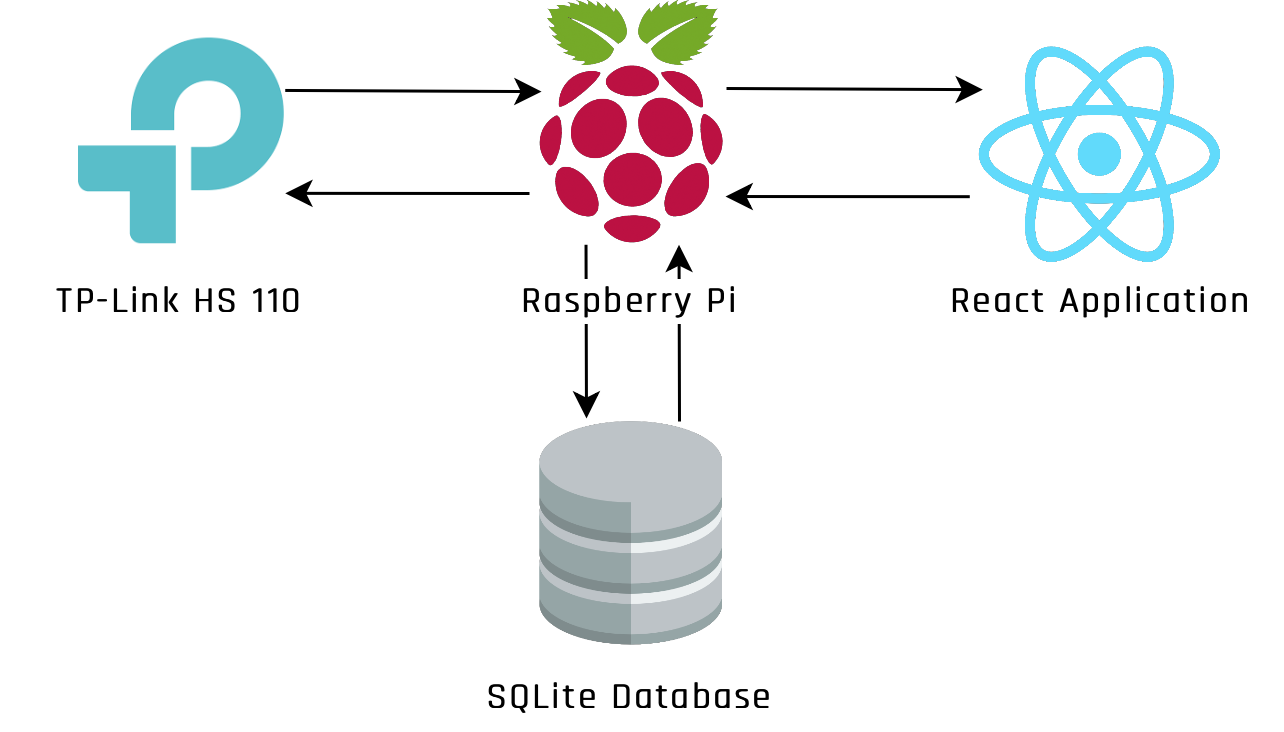
\includegraphics[width=0.8\textwidth]{Figures/AppDesign.png}
	\caption{Schématický návrh komunikace jednotlivých částí aplikace a zařízení}
	\label{fig:AppDesign}
\end{figure}

\clearpage

\subsection{Backend aplikace}
Backendová aplikace běžící na Raspberry Pi je logicky rozdělena do 4 částí napsaných v .NET Core 3.1, jazyce \texttt{C\#}. Konkrétně se jedná o:

\begin{itemize}
\item \textbf{SmartPlugORM:}
Je knihovnou vytvořenou pro objektově relační mapování\autocite{PofEAA}, která zajišťuje jednoduché operace nad SQLite databází, jako je vkládání nových záznamů nebo načítání dat z databáze a automatickou konverzi entit na objekty. Je použita v následujících dvou aplikacích pro získávání dat a jejich poskytování. Díky tomu odpadá potenciální problém s duplicitou kódu napříč aplikacemi. Pro ukládání záznamů o měření spotřeby z chytré zásuvky postačuje jednoduchá tabulka obsahující veličiny související s měřením, datum s časem vytvoření záznamu a jeho identifikátor. Strukturu tabulky je možno vidět v následující tabulce \ref{tab:Table emeter}:

\bigbreak

\begin{table}[ht!]
	\centering
	\begin{tabular}{lccc}
		\hline
		Název & Datový typ & Klíč & Null \\
		\hline
		id & integer & Primární & Ne \\
		voltage & integer & Ne & Ne \\
		current & integer & Ne & Ne \\
		power & integer & Ne & Ne \\
		created_at & datetime & Ne & Ne \\
		\hline
	\end{tabular}
	\caption{Tabulka emeter}
	\label{tab:Table emeter}
\end{table}

\item \textbf{SmartPlugDataCollector:}
Je konzolová aplikace, využívající knihovnu \texttt{SmartPlugORM}, spuštěná jako služba na Raspberry Pi, která periodicky každé 4 minuty zasílá příkaz na chytrou zásuvku s požadavkem o vrácení aktuálních údajů o spotřebě. Takovýto příkaz vypadá před šifrováním následovně:
\bigbreak
\begin{lstlisting}[language=json,caption=TP-Link HS110 příkaz pro získání okamžitých údajů o spotřebě]
{
	"emeter": {
		"get_realtime": {},
		"get_vgain_igain": {}
	}
}
\end{lstlisting}
\bigbreak
\noindent Šifrování zpráv pak probíhá tak, že se první byte zprávy zašifruje bitovou operací \texttt{XOR} a hodnotou \texttt{0xAB}. Následující byte se pak šifruje hodnotou předchozího zašifrovaného bytu. Pro dešifrování platí analogicky obdobné pravidlo s tím rozdílem, že se jako následující klíč volí hodnota bytu před dešifrováním. Tomuto přístupu se také říká autoklíčová šifra. K odhalení tohoto způsobu šifrování můžeme využít zpětného inženýrství, například dekompilace Android aplikace Kasa\autocite{KASA}.

\item \textbf{SmartPlugAPI:}
Je ASP.NET Core webová aplikace, využívající knihovnu \texttt{SmartPlugORM}, která je spuštěna také jako služba na Raspberry Pi. Obsahuje dvě následující HTTP GET metody:
\begin{itemize}
	\item \textbf{GetAll} – Vrací veškeré naměřené záznamy ve formátu JSON. Ukázku odpovědi je možno vidět ve výpise \ref{lst:api}.
	\item \textbf{GetByDate} – Vrací naměřené záznamy v zadaném rozsahu dat. Obsahuje dva povinné parametry \texttt{fromDate} a \texttt{toDate}. Tyto parametry musí dodržet normu ISO 8601, která definuje formát pro zápis data a času.
\end{itemize}
\noindent Cesty k těmto endpointům jsou přistupné ve formátu \texttt{"/api/emeter/METODA"}.
\bigbreak
\begin{lstlisting}[language=json,caption=Ukázka odpovědi aplikačního rozhraní,label={lst:api}]
[
	{
		"voltage": 235013,
		"current": 13,
		"power": 0,
		"createdAt": "2020-11-08T13:05:10"
	},
	...
],
\end{lstlisting}

\item \textbf{SmartPlugTests:}
Obsahuje unit testy testující funkcionalitu výše zmíněného šifrování a dešifrování. Dále zahrnuje také testování API metody pro získávání záznamů podle data.
		
\end{itemize}

\bigbreak
\noindent Schématickou reprezentaci závislostí mezi moduly v projektu je možno vidět na obrázku \ref{fig:ProjectDependency}.

\bigbreak

\begin{figure}[h!]
	\centering
	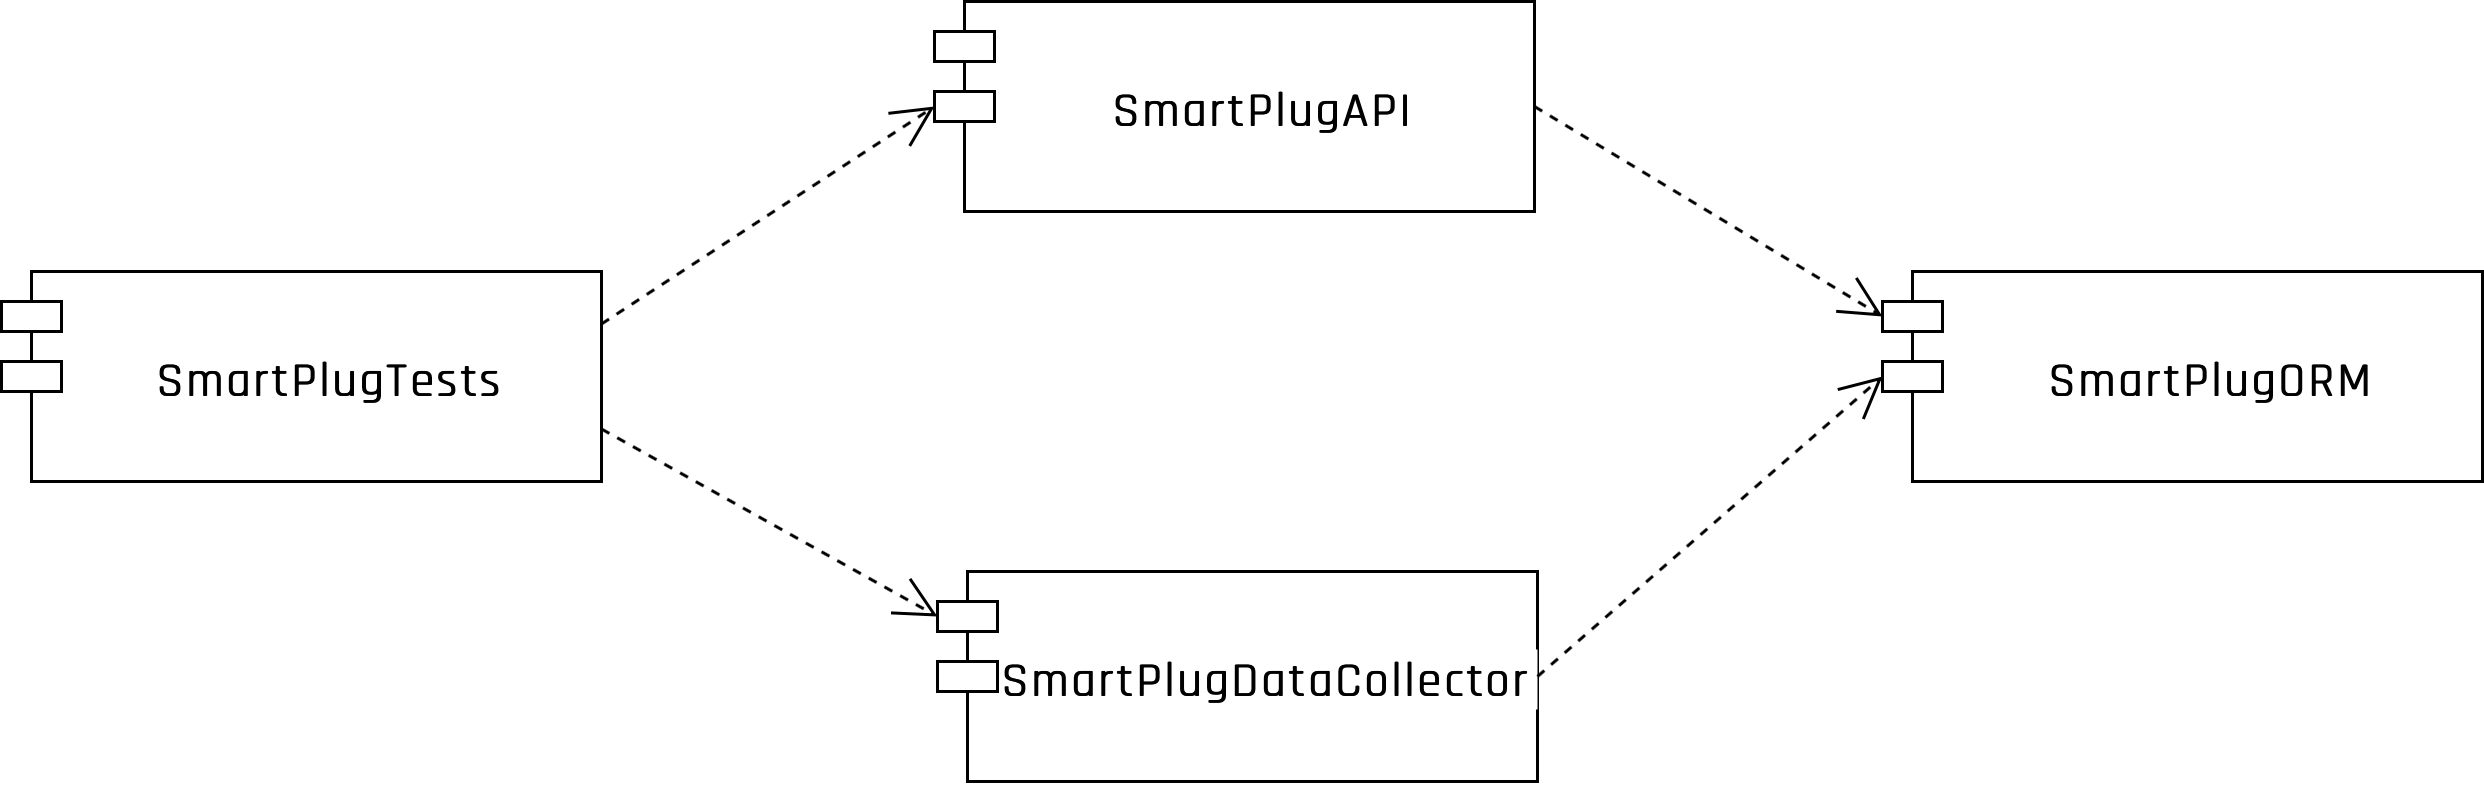
\includegraphics[width=1\textwidth]{Figures/ProjectDependency.png}
	\caption{Schématická reprezentace závislostí jednotlivých modulů}
	\label{fig:ProjectDependency}
\end{figure}

\pagebreak

\subsection{Nasazení na Raspberry Pi}
Pro spuštění a nepřetržitý provoz vytvořených aplikaci bylo nutné Raspberry Pi nejdříve připravit. Což znamenalo kromě samotného nainstalování operačního systému Raspbian také povolit SSH pro vzdálený přístup, instalaci \texttt{SQLite} a vytvoření databázové struktury zmíněné výše\ref{tab:Table emeter}. Dále také instalaci \texttt{.NET Core SDK 3.1} včetně \texttt{ASP.NET Core Runtime 3.1 } a registrovat cestu k nim do proměnných prostředí (environment variables). V případě, že by bylo nutné systém restartovat, bylo potřeba tyto cesty přidat do souboru \texttt{.profile}:
\bigbreak
\begin{lstlisting}[language=bash,caption=Proměnné prostředí pro cesty k .NET Core SDK a ASP.NET Runtime]
export DOTNET_ROOT=$HOME/dotnet-arm32
export PATH=$PATH:$HOME/dotnet-arm32
\end{lstlisting}
\bigbreak
Po úspěšném otestování balíčků, například příkazem \texttt{dotnet --info}, bylo následně možné přesunout již vytvořené aplikace pomocí protokolu SSH, příkazem \texttt{scp} na Raspberry Pi a spustit je příkazem \texttt{dotnet SmartPlugDataCollector} a \texttt{dotnet SmartPlugApi}. Pro otestování funkčnosti bylo možné přistoupit na endpoint vytvořeného API pod IP adresou zařízení v místní síti. V této fázi by bylo možné začít implementovat frontendovou aplikaci, nicméně pokud by bylo nutné zařízení restartovat v případě výpadku sítě, elektrického napájení nebo jiného problému, bylo vhodné tyto aplikace zaregistrovat jako služby, které se automaticky v případě havárie restartují nebo spustí při startu systému. K tomu bylo potřeba vytvořit nové démony \texttt{/etc/systemd/system/smart-plug-data-collector.service} a \texttt{/etc/systemd/system/smart-plug-api.service}. Konfiguraci služby pro \texttt{SmartPlugAPI} je možno vidět v ukázce. Služba pro \texttt{SmartPlugDataCollector} byla konfigurována analogicky obdobným způsobem. 
\bigbreak
\begin{lstlisting}[language={},caption=Konfigurace jedné z aplikací jako systémové služby]
[Unit]
Description=ASP.NET Core 3.1 App - SmartPlugAPI

[Service]
WorkingDirectory=/home/pi/smartplug
ExecStart=/home/pi/dotnet-arm32/dotnet /home/pi/smartplug/SmartPlugAPI.dll
Restart=always
RestartSec=10
KillSignal=SIGINT
SyslogIdentifier=dotnet-SmartPlugAPI
User=pi
Environment=ASPNETCORE_ENVIRONMENT=Production
Environment=DOTNET_PRINT_TELEMETRY_MESSAGE=false

[Install]
WantedBy=multi-user.target
\end{lstlisting}

\begin{lstlisting}[language=bash,caption=Povolení a start služby]
sudo systemctl enable smart-plug-api.service
sudo systemctl start smart-plug-api.service
sudo systemctl status smart-plug-api.service
\end{lstlisting}

\noindent Po úspěšném startu služby byl vidět v konzoli aktivní stav a aplikační rozhraní v prohlížeči stále funguje, tudíž bylo možné přejít k implementaci frontendové části aplikace.

\pagebreak
\subsection{Frontend aplikace} 
Celá frontendová část projektu byla tvořena jako single-page aplikace s použitím knihovny \texttt{React} využívající výše zmíněné aplikační rozhraní. Kromě knihoven pro grafové vizualizace zde byla použita knihovna \texttt{Material-UI}\autocite{MaterialUI} pro některé prvky uživatelského rozhraní. Dále také knihovna \texttt{axios}\autocite{axios} pro usnadnění AJAX komunikace s API.

Webové rozhraní obsahuje několik prvků pro interakci s uživatelem. Nejdůležitější z nich jsou pole pro výběr časového úseku \texttt{From} a \texttt{To}, který má být analyzován a vizualizován. Podle hodnot těchto vstupů je následně zaslán požadavek na API. Data z odpovědi jsou pak zpracována a vizualizována pomocí grafů. Dále obsahuje tři zaškrtávací políčka pro filtraci elektrických veličin zobrazených v hlavním grafu. V levém sloupci je možno vidět vypočtené statistiky z naměřených dat. Nad hlavním grafem se nachází kromě první záložky také další dvě, ve které obsahují vstupní pole pro parametry shlukovacích algoritmů \texttt{K-Means} a \texttt{DBSCAN}, na jejichž základě je proveden výpočet s vybraným časovým úsekem dat a vizualizací shluků. Ukázku prvního pohledu na aplikaci je možno vidět na obrázku \ref{fig:React1}.

\bigbreak
\begin{figure}[h!]
	\centering
	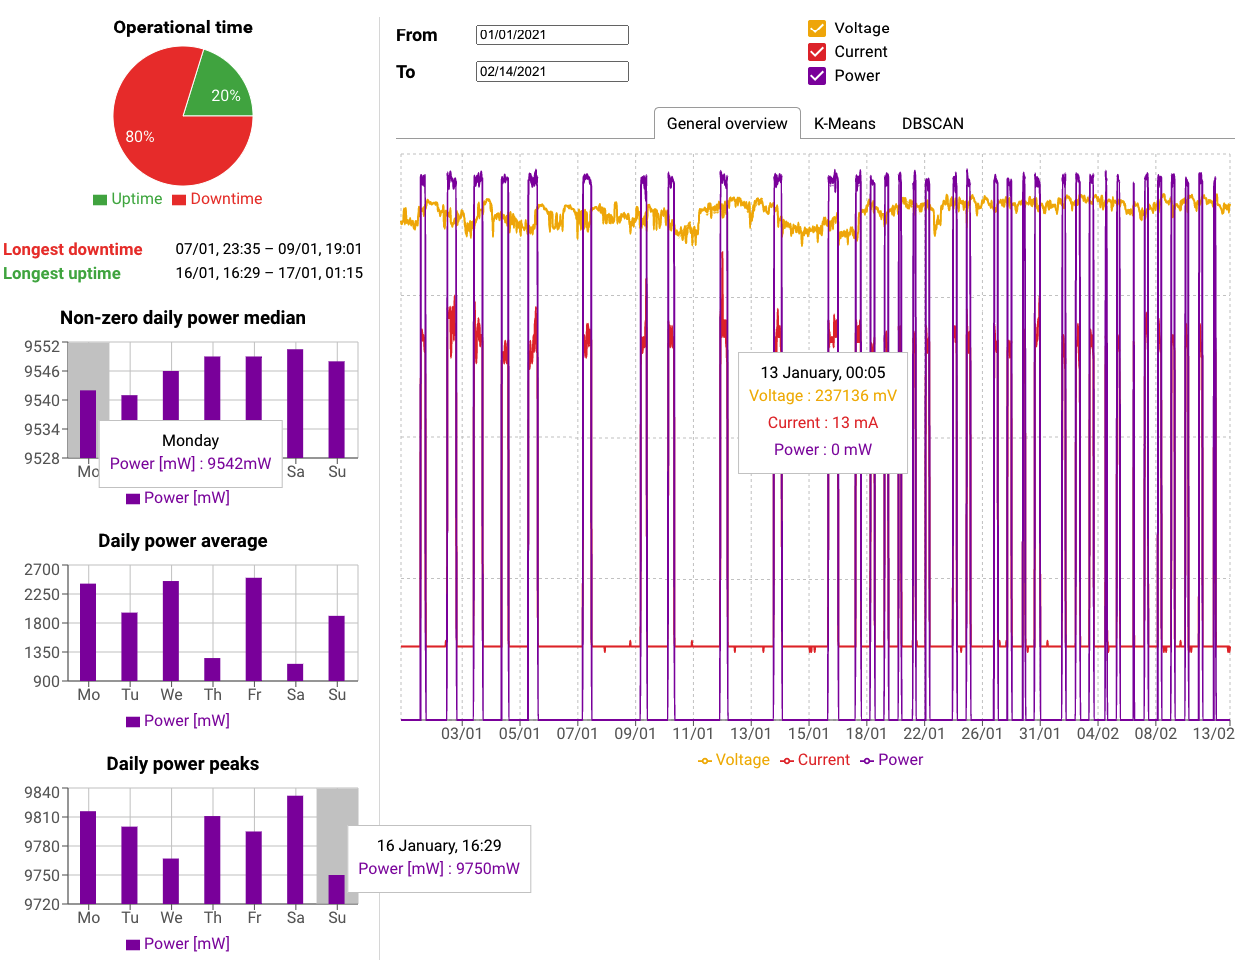
\includegraphics[width=1\textwidth]{Figures/React1.png}
	\caption{Ukázka vizualizace časového průběhu elektrických veličin a statistik}
	\label{fig:React1}
\end{figure}
\pagebreak

Struktura aplikace je členěna do několika komponent, z nichž některé jsou použity v rámci aplikace několikrát. Jedná se například o sloupcové grafy, které je možno vidět v levém sloupci se statistikami a jejich odlišnosti při použití jsou řešeny skrze předávání parametrů pomocí \texttt{props}. Většina logiky pro zpracování dat se nachází mimo samotné React komponenty v souboru \texttt{utils.js}, případně samostatném JavaScript souboru pro jednotlivé shlukovací algoritmy.

\subsubsection*{Komponenty pro analýzu dat a jejich vizualizaci}
\begin{itemize}
	\item \textbf{General overview} – Jedná se o obecný spojnicový graf zobrazující v čase jednotlivé naměřené elektrické veličiny ve zvoleném rozsahu, tyto veličiny je možno filtrovat pomocí zaškrtávacích políček. Viz obrázek \ref{fig:React1}.
	\item \textbf{Operational time}	– Reprezentuje v koláčovém grafu poměr času, kdy bylo zařízení zapnuté a vypnuté. Kromě toho také detekuje nejdelší dobu po kterou bylo zařízení zapnuté a vypnuté. Tu zobrazuje v textové podobě. Viz obrázek \ref{fig:React1}.
	\item \textbf{Non-zero daily power consumption median} – Představuje sloupcový graf obsahující denní mediány z nenulových naměřených hodnot spotřeby. Nenulových z toho důvodu, že měřené zařízení bylo většinu času vypnuté, proto by výsledky ze kompletních naměřených hodnot byly irelevantní. Viz obrázek \ref{fig:React1}.
	\item \textbf{Daily power average} – Jedná se o sloupcový graf vizualizující průměry okamžitých hodnot elektrické spotřeby z chytré zásuvky v rámci dnů v týdnu. Viz obrázek \ref{fig:React1}.
	\item \textbf{Daily power peaks} – Reprezentuje v sloupcovém grafu píky okamžité elektrické spotřeby za každý den v týdnu. Při najetí myši na konkrétní den se zobrazí plovoucí okno, ve kterém se nachází přesný datum a čas kdy k píku došlo. Viz obrázek \ref{fig:React1}.
	\pagebreak
	\item \textbf{K-Means} – Představuje shlukovací algoritmus jehož vstupem je kromě dat pouze počet shluků – \texttt{K}. Algoritmus funguje tak, že v prvním kroku zvolí náhodně počáteční centroidy jednotlivých shluků. Poté postupuje iterativně tak, že v každém kroku přiřazuje k jednotlivým shlukům objekty podle jejich vzdálenosti od centroidů tak dlouho, dokud nedojde k žádné záměně. Při aplikaci tohoto algoritmu byla jako data využity průměrné hodinové spotřeby v rámci dnů. Pro určení vzdálenosti byla použita Euklidovská metrika. Vizualizovaný výsledek je možno vidět na obrázku \ref{fig:React2}.
	\begin{figure}[h!]
		\centering
		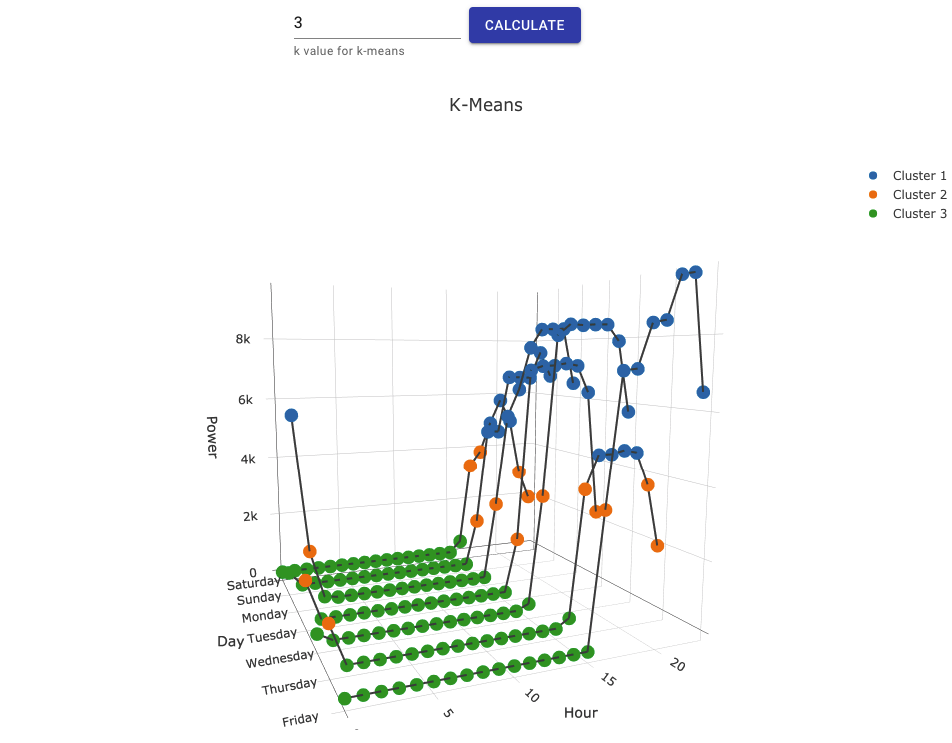
\includegraphics[width=1\textwidth]{Figures/React2.png}
		\caption{Ukázka vizualizace výsledků shlukovacího algoritmu K-Means}
		\label{fig:React2}
	\end{figure}
	\pagebreak
	\item \textbf{DBSCAN} (Density-based spatial clustering of applications with noise) – Jedná se o další shlukovací algoritmus, který vyžaduje dva parametry: Vzdálenost $\epsilon$ a minimální počet objektů nutný pro zformování shluku. Algoritmus funguje tak, že pro každý objekt je počítáno počet objektů v jeho $\epsilon$ okolí. Pokud splní požadavek na minimální počet objektů pro zformování shluku, je vytvořen nový shluk a následně jsou do něj přiřazeny také ty objekty, které jsou dosažitelné v rámci $\epsilon$ vzdálenosti z tzv. \texttt{core points}, tudíž takových objektů v shluku, jejichž počet sousedů je alespoň roven minimálnímu počtu objektů na shluk definovaným na počátku algoritmu. V opačném případě jsou objekty označeny jako šum. Ukázku výsledku algoritmu je možno vidět na obrázku \ref{fig:React3}. Obdobně jako u K-Means je zde použita stejná metrika a data jsou předpřipravená stejným způsobem.
	\begin{figure}[h!]
		\centering
		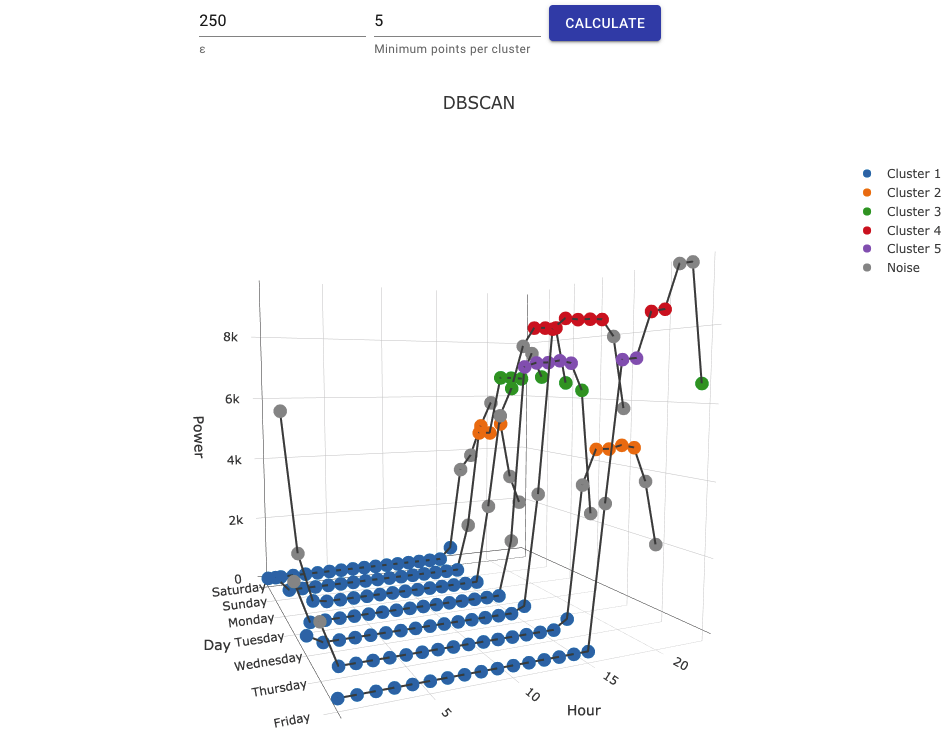
\includegraphics[width=1\textwidth]{Figures/React3.png}
		\caption{Ukázka vizualizace výsledků shlukovacího algoritmu DBSCAN}
		\label{fig:React3}
	\end{figure}
\end{itemize}

\pagebreak 

Pro shlukovací algoritmy se ve webovém rozhraní také nachází textová podoba výsledků s jednotlivými skupinami objektů, které jsou si, z hlediska hodinových průměrů okamžité spotřeby v rámci dnů v týdnu, podobné. Viz obrázek \ref{fig:React4}.

\begin{figure}[h!]
	\centering
	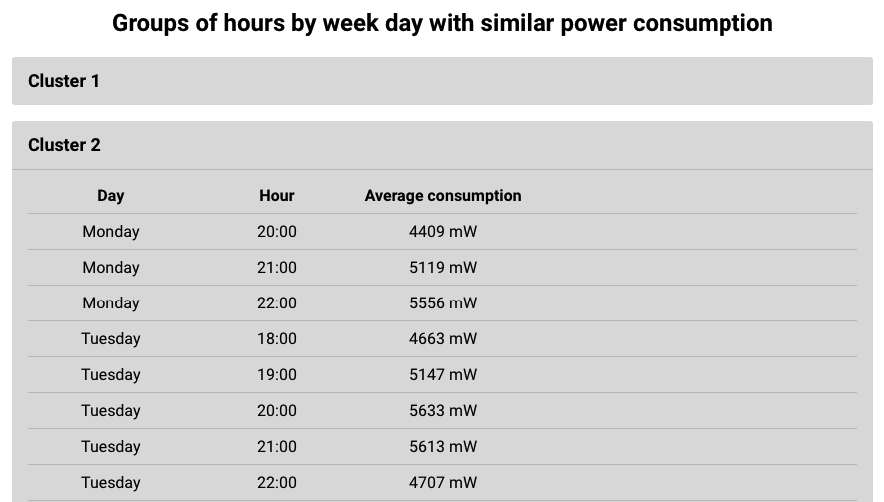
\includegraphics[width=1\textwidth]{Figures/React4.png}
	\caption{Ukázka textové reprezentace výsledků shlukovacích algoritmů}
	\label{fig:React4}
\end{figure}

\pagebreak
\section{Závěr}
Jako výsledek práce na projektu se mi podařilo vytvořit tři vzájemně propojené aplikace, které se starají o automatizovaný sběr dat z chytré zásuvky a ukládání do databáze, jejich následné poskytování skrze aplikační rozhraní a jeho využití v React aplikaci, která se stará o vizualizaci dat a výpočet statistik. Kromě toho také obsahuje vizualizaci výsledků některých shlukovacích algoritmů.

Díky práci na tomto projektu jsem si mohl rozšířit své znalosti v oblastech tvorby React aplikací, asynchronní ko vybírármunikací s aplikačním rozhraním a prací s grafovými knihovnami. Zcela novou problematikou pro mne byla práce s Raspberry Pi a komunikace s chytrým zařízením.

\clearpage

\nocite{*}
\printbibliography[title={Literatura}, heading=bibintoc]
%\appendix

\end{document}
